\documentclass[11pt,a4paper]{article}
\usepackage[textwidth=37em,vmargin=30mm]{geometry}
\usepackage{calc,xunicode,amsmath,amssymb,paralist,enumitem,tabu,booktabs,datetime2,xeCJK,xeCJKfntef,listings}
\usepackage{tocloft,fancyhdr,tcolorbox,xcolor,graphicx,eso-pic}

\usepackage[hidelinks]{hyperref}
\hypersetup{
    colorlinks=false,
    pdfpagemode=FullScreen,
    pdftitle={Web Digest - 2023-01-07}
}

\setdefaultleftmargin{2em}{2em}{1em}{1em}{1em}{1em}

\usepackage{xeCJK,xeCJKfntef}
\newcommand{\myvphantom}[0]{\vphantom{QWERTYUIOPASDFGHJKLZXCVBNMqwertyuiopasdfghjklzxcvbnm1234567890ςρθδφγηξλζχψβμ\"A}}
\xeCJKsetup{PunctStyle=plain,RubberPunctSkip=false,CJKglue=\myvphantom\hskip 0pt plus 0.1em minus 0.05em,CJKecglue=\myvphantom\hskip 0.22em plus 200pt}
\XeTeXlinebreaklocale "zh"
\XeTeXlinebreakskip = 0pt


\setmainfont[Numbers=Lining]{Brygada 1918}
\setromanfont[Numbers=Lining]{Brygada 1918}
\setsansfont[Numbers=Lining]{IBM Plex Sans}
\setmonofont{JetBrains Mono NL}
\setCJKmainfont{Noto Serif CJK SC}
\setCJKromanfont{Noto Serif CJK SC}
\setCJKsansfont{Noto Sans CJK SC}
\setCJKmonofont{Noto Sans CJK SC}

\setlength{\parindent}{0pt}
\setlength{\parskip}{8pt}
\linespread{1.15}

\lstset{
	basicstyle=\ttfamily\footnotesize,
	numbersep=5pt,
	backgroundcolor=\color{black!5},
	showspaces=false,
	showstringspaces=false,
	showtabs=false,
	tabsize=2,
	captionpos=b,
	breaklines=true,
	breakatwhitespace=true,
	breakautoindent=true,
	linewidth=\textwidth
}






\newcommand{\coverpic}[2]{
    % argv: itemurl, authorname
    Cover photo by #2~~~~(\href{#1}{#1})
}
\newcommand{\makeheader}[0]{
    \begin{center}
        
        \rmfamily\scshape
        \fontsize{62pt}{70pt}\selectfont
        WEB\hfill DIGEST
        
        \vfill
        % \vskip 30pt
        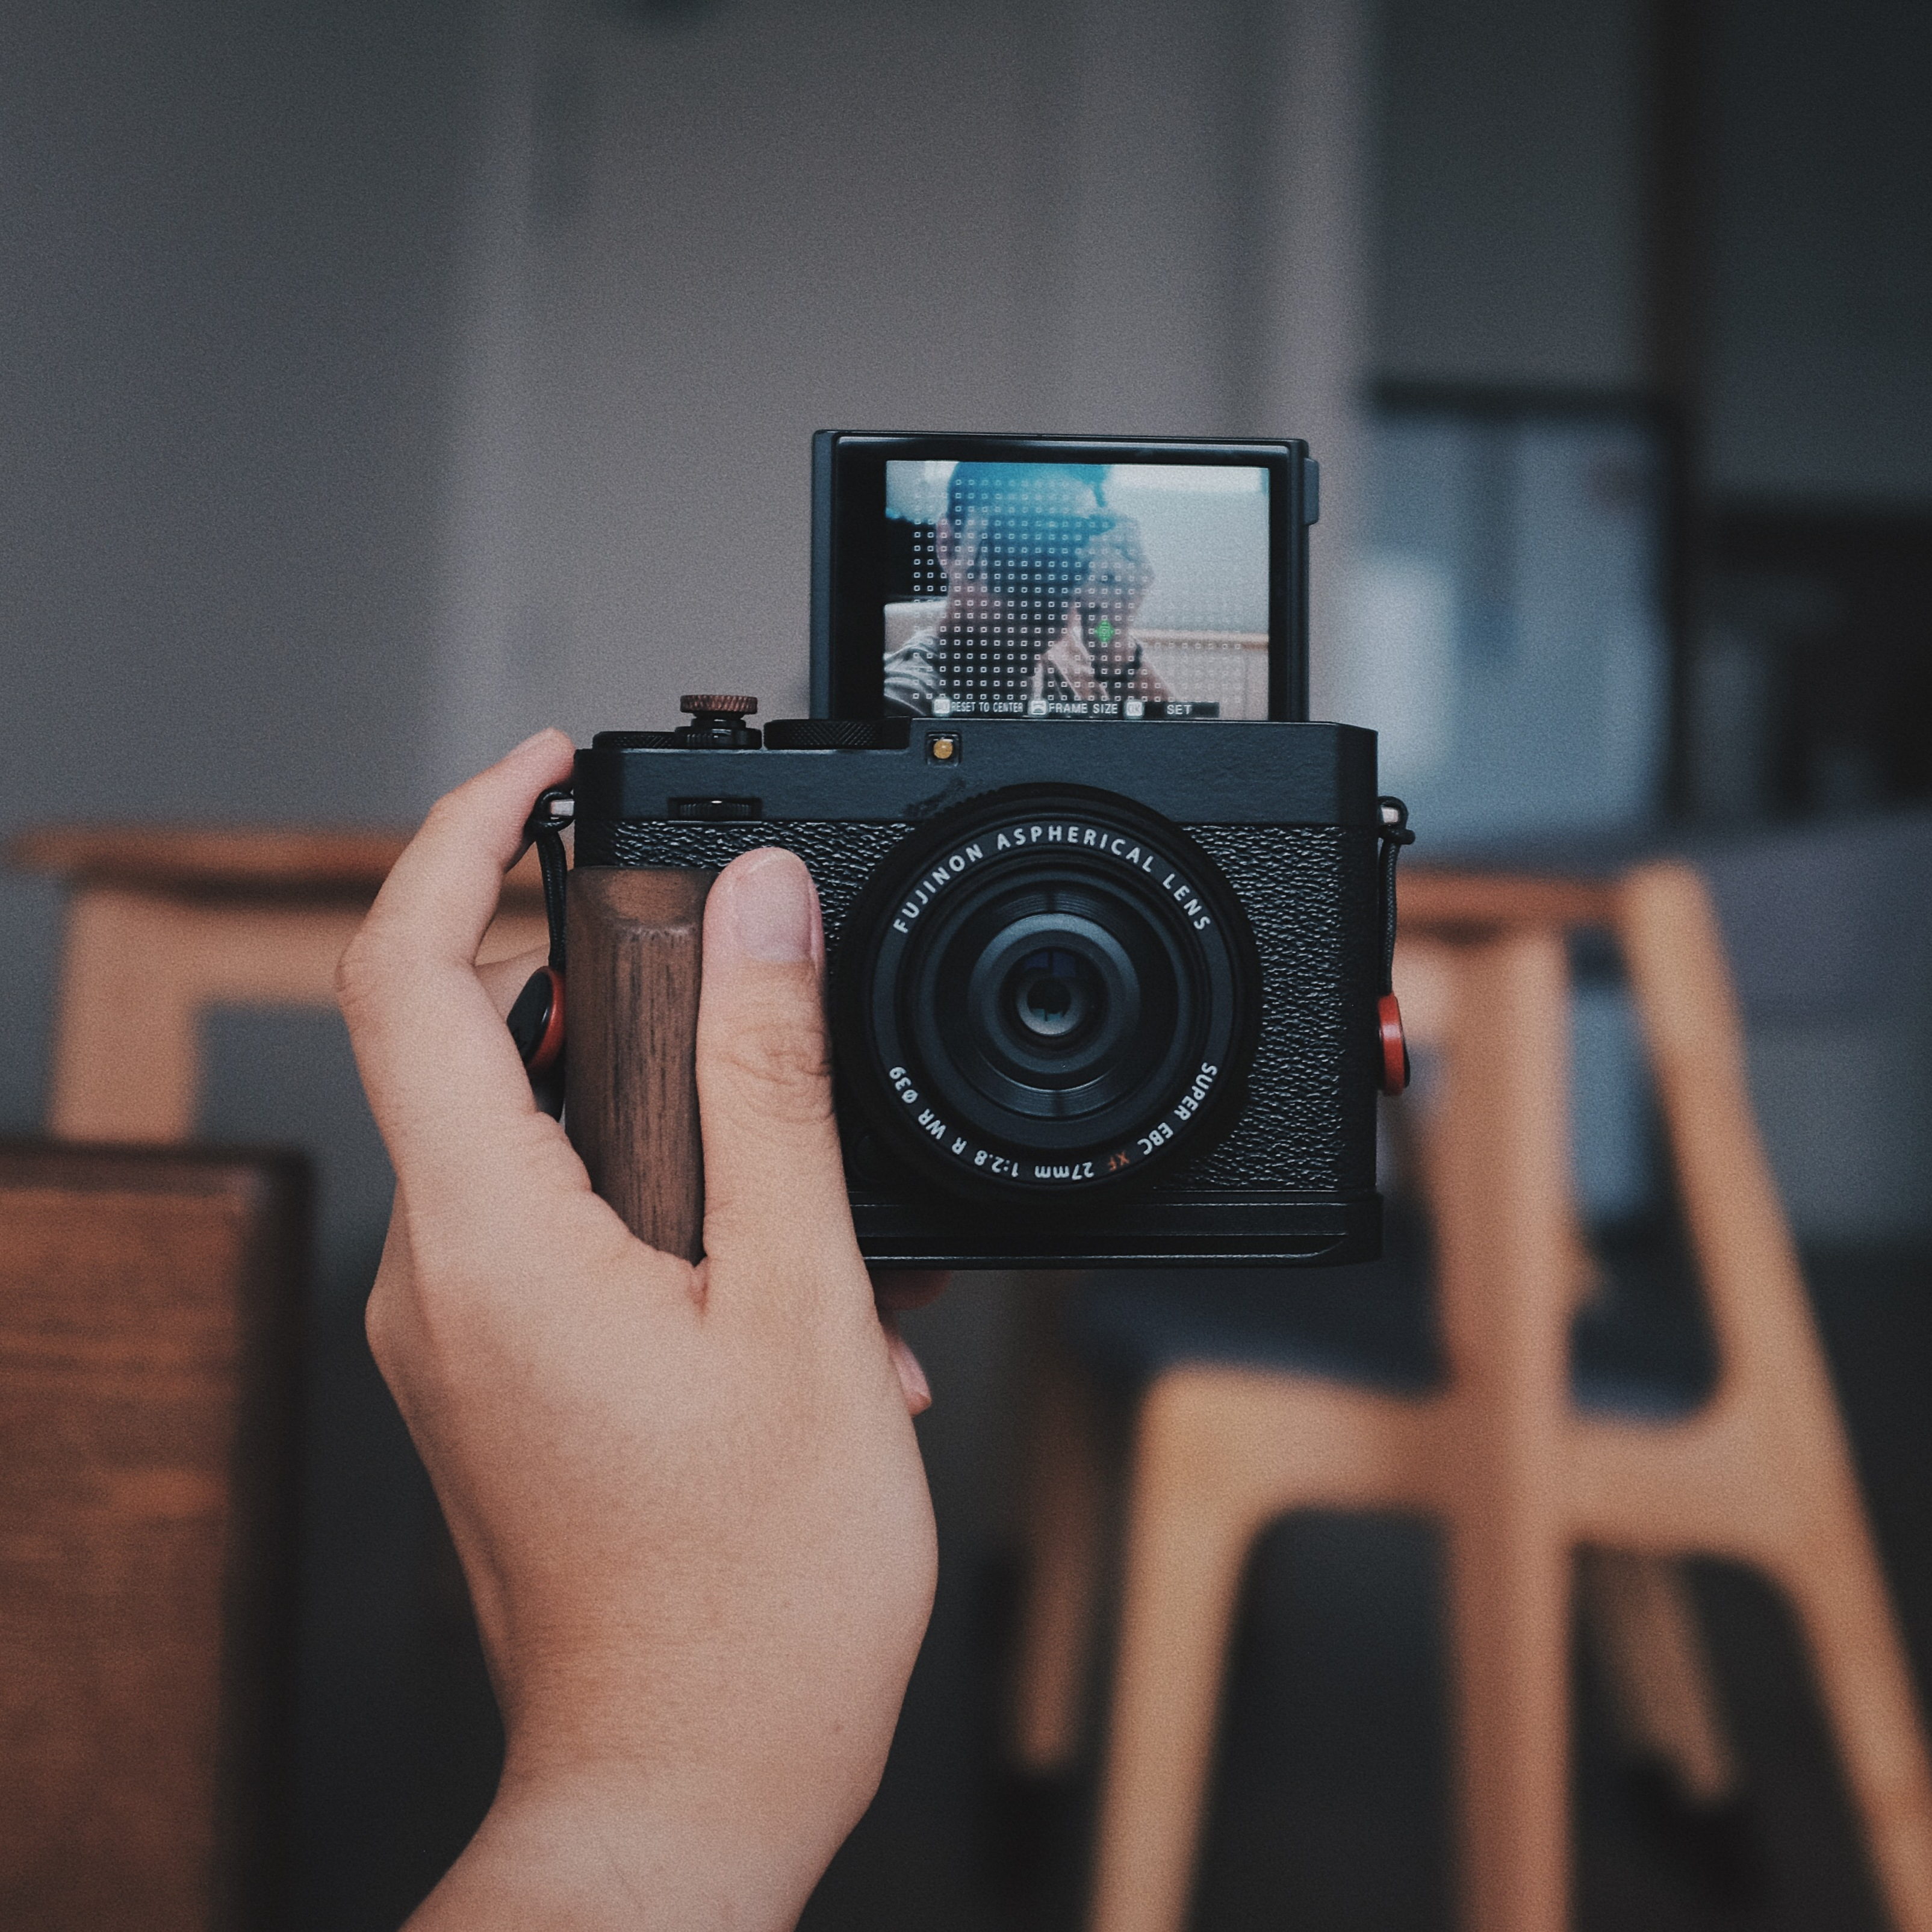
\includegraphics[width=\linewidth]{./webdb/2023/20230107/final/coverpic.jpg}\par
        % \vskip 30pt
        \vfill

        \normalsize\upshape
        \copyright{} The Web Digest Project \hfill\large 2023-01-07
    \end{center}
    % \vskip 20pt
    % \hrule
    % \vskip 10pt
    % \clearpage
}
\renewcommand{\contentsname}{\Huge\sffamily\bfseries Contents\par\vskip 20pt}
\newcounter{ipartcounter}
\setcounter{ipartcounter}{0}
\newcommand{\ipart}[1]{
    % \vskip 20pt
    \clearpage
    \stepcounter{ipartcounter}
    \phantomsection
    \addcontentsline{toc}{section}{#1}
    \begin{center}
        \Huge
        \sffamily\bfseries
        #1
    \end{center}
    \vskip 20pt
}
\newcommand{\entryitemHackernews}[3]{
    % argv: title, hnurl, rawurl
    \parbox{\linewidth}{
        \Large\rmfamily\bfseries#1\par\vskip 5pt
        \footnotesize\ttfamily\mdseries
        \href{#3}{#3}\par
        \textcolor{black!50}{\href{#2}{#2}}\par
    }\vskip 11pt
}
\newcommand{\entryitemGeneric}[2]{
    % argv: title, url
    \parbox{\linewidth}{
        \Large\rmfamily\bfseries#1\par\vskip 5pt
        \footnotesize\ttfamily\mdseries
        \href{#2}{#2}\par
    }\vskip 11pt
}






\begin{document}

\begin{titlepage}
	\makeheader
\end{titlepage}

\tableofcontents\clearpage


\ipart{Hacker News}
\entryitemHackernews{\hskip 0pt{}Universal flu vaccine against all known subtypes takes promising first steps}{https://news.ycombinator.com/item?id=34289092}{https://www.science.org/doi/10.1126/science.abm0271}

\entryitemHackernews{\hskip 0pt{}I've realized I'm a bad software developer}{https://news.ycombinator.com/item?id=34288229}{https://gaylelaakmann.substack.com/p/ive-realized-im-a-bad-software-developer}

\entryitemHackernews{\hskip 0pt{}Rsync.net warrant canary}{https://news.ycombinator.com/item?id=34287964}{https://www.rsync.net/resources/notices/canary.txt}

\entryitemHackernews{\hskip 0pt{}Study Finds That Buttons in Cars Are Safer and Quicker to Use Than Touchscreens}{https://news.ycombinator.com/item?id=34287800}{https://futurism.com/the-byte/study-finds-that-buttons-in-cars-are-safer-and-quicker-to-use-than-touchscreens}

\entryitemHackernews{\hskip 0pt{}Not-such-better-living through chemistry}{https://news.ycombinator.com/item?id=34287564}{https://www.science.org/content/blog-post/not-such-better-living-through-chemistry}

\entryitemHackernews{\hskip 0pt{}Modern C for C++ Peeps (2019)}{https://news.ycombinator.com/item?id=34287562}{https://floooh.github.io/2019/09/27/modern-c-for-cpp-peeps.html}

\entryitemHackernews{\hskip 0pt{}Tell HN: Vim users, `:x` is like `:wq` but writes only when changes are made}{https://news.ycombinator.com/item?id=34287407}{https://news.ycombinator.com/item?id=34287407}

\entryitemHackernews{\hskip 0pt{}The beauty of CGI and simple design}{https://news.ycombinator.com/item?id=34286622}{https://rubenerd.com/the-beauty-of-cgi-and-simple-design-by-hales/}

\entryitemHackernews{\hskip 0pt{}Software horror show: SAP Concur}{https://news.ycombinator.com/item?id=34286122}{https://blog.plover.com/prog/crap-warning-signs-2.html}

\entryitemHackernews{\hskip 0pt{}Epochalypse}{https://news.ycombinator.com/item?id=34284759}{https://www.epochalypse.today/}

\entryitemHackernews{\hskip 0pt{}Monkey stone tools shed doubts on the human origin of archeological sites}{https://news.ycombinator.com/item?id=34283861}{https://journals.sagepub.com/doi/10.1177/09596836221131707}

\entryitemHackernews{\hskip 0pt{}Death by vegetable oil: What the studies say (2020)}{https://news.ycombinator.com/item?id=34283427}{https://www.jeffnobbs.com/posts/death-by-vegetable-oil-what-the-studies-say}

\entryitemHackernews{\hskip 0pt{}Physical buttons outperform touchscreens in new cars, test finds (2022)}{https://news.ycombinator.com/item?id=34283385}{https://www.vibilagare.se/english/physical-buttons-outperform-touchscreens-new-cars-test-finds}

\entryitemHackernews{\hskip 0pt{}Less gym time, same results: Why `lowering' weights is all you need to do}{https://news.ycombinator.com/item?id=34282662}{https://www.ecu.edu.au/newsroom/articles/research/less-gym-time-same-results-why-lowering-weights-is-all-you-need-to-do}

\entryitemHackernews{\hskip 0pt{}Things they didn't teach you about software engineering}{https://news.ycombinator.com/item?id=34282339}{https://vadimkravcenko.com/shorts/things-they-didnt-teach-you/}

\entryitemHackernews{\hskip 0pt{}Why didn't we get the four-hour workday?}{https://news.ycombinator.com/item?id=34281474}{https://rootsofprogress.org/the-four-hour-workday-prediction}

\entryitemHackernews{\hskip 0pt{}Perfect Circle}{https://news.ycombinator.com/item?id=34280708}{https://neal.fun/perfect-circle/}

\entryitemHackernews{\hskip 0pt{}Why was Roman concrete so durable?}{https://news.ycombinator.com/item?id=34280239}{https://news.mit.edu/2023/roman-concrete-durability-lime-casts-0106}

\entryitemHackernews{\hskip 0pt{}Ask HN: Share your personal site}{https://news.ycombinator.com/item?id=34279215}{https://news.ycombinator.com/item?id=34279215}

\entryitemHackernews{\hskip 0pt{}Ask HN: What \$500-2500 product improved your 2022}{https://news.ycombinator.com/item?id=34279146}{https://news.ycombinator.com/item?id=34279146}

\ipart{V2EX}
\entryitemGeneric{\hskip 0pt{}[macOS] mac 把文件从内置硬盘移动到移动硬盘,发现写入算内置硬盘?}{https://www.v2ex.com/t/907289}

\entryitemGeneric{\hskip 0pt{}[程序员] React Native 可以精简大小吗?在 Android 下默认就 55MB 了}{https://www.v2ex.com/t/907288}

\entryitemGeneric{\hskip 0pt{}[深圳] 有没有 14-15 号深圳回南阳的车, 2 个位。火车抢不到哇}{https://www.v2ex.com/t/907287}

\entryitemGeneric{\hskip 0pt{}[宽带症候群] 成都电信组播看 iptv}{https://www.v2ex.com/t/907285}

\entryitemGeneric{\hskip 0pt{}[分享创造] 开源 C 库实现 HTTP 服务器:多线程+事件模型+外挂式跟踪技术}{https://www.v2ex.com/t/907284}

\entryitemGeneric{\hskip 0pt{}[Apple] 马区 Apple One 中杯订阅合租季付}{https://www.v2ex.com/t/907282}

\entryitemGeneric{\hskip 0pt{}[京东] 1.8 京东 PLUS 超级联名卡又开启耍猴模式}{https://www.v2ex.com/t/907280}

\entryitemGeneric{\hskip 0pt{}[问与答] 如何快速删除我所有的微信收藏?}{https://www.v2ex.com/t/907279}

\entryitemGeneric{\hskip 0pt{}[Java] 新手请教各位前辈 关于换项目和新技术的学习}{https://www.v2ex.com/t/907278}

\entryitemGeneric{\hskip 0pt{}[问与答] 微信支付的小微商户收款只能通过第三方来申请?}{https://www.v2ex.com/t/907277}

\entryitemGeneric{\hskip 0pt{}[前端开发] 使用 Taro 来构建一个小程序组件库,有什么可以抄作业的最佳实践吗?}{https://www.v2ex.com/t/907276}

\entryitemGeneric{\hskip 0pt{}[Apple] 现在 iPhone 无法关闭双重验证了吗}{https://www.v2ex.com/t/907275}

\entryitemGeneric{\hskip 0pt{}[分享发现] 各位城市最近行车状况如何,我感觉越临近过年,乱插的车越多}{https://www.v2ex.com/t/907274}

\entryitemGeneric{\hskip 0pt{}[分享发现] 《朗文当代高级英语词典》mac 版,适配原生 Dictionary APP}{https://www.v2ex.com/t/907272}

\entryitemGeneric{\hskip 0pt{}[macOS] 破案 Tab 键在 Safari 中刷题不是空格而是键盘巡航功能}{https://www.v2ex.com/t/907271}

\entryitemGeneric{\hskip 0pt{}[Windows] Microsoft store 老是出现``假更新''}{https://www.v2ex.com/t/907269}

\entryitemGeneric{\hskip 0pt{}[分享发现] 最近接触到 matrix 网桥,创建了一个通过 matrix 桥接 tg 和 discord 的联合群组,有兴趣的可以加入}{https://www.v2ex.com/t/907267}

\entryitemGeneric{\hskip 0pt{}[英雄联盟] 台服 LOL 也有 mac 版了}{https://www.v2ex.com/t/907266}

\entryitemGeneric{\hskip 0pt{}[程序员] 有接私活的吗 来一个}{https://www.v2ex.com/t/907265}

\entryitemGeneric{\hskip 0pt{}[程序员] PerimeterX 的按压验证 咋这么牛}{https://www.v2ex.com/t/907264}

\entryitemGeneric{\hskip 0pt{}[哔哩哔哩] 请教成功经验,怎么减少看 b 站?}{https://www.v2ex.com/t/907263}

\entryitemGeneric{\hskip 0pt{}[Apple] airpods 和 win11 的兼容性问题}{https://www.v2ex.com/t/907261}

\entryitemGeneric{\hskip 0pt{}[宽带症候群] 杭州电信 ipv6, tracert 二跳就丢包运营商问题吗}{https://www.v2ex.com/t/907260}

\entryitemGeneric{\hskip 0pt{}[分享创造] Tailchat v1.4.0 已发布,欢迎试用}{https://www.v2ex.com/t/907259}

\entryitemGeneric{\hskip 0pt{}[程序员] 为什么 npm 包不要求把包作者也写到依赖中去?}{https://www.v2ex.com/t/907258}

\entryitemGeneric{\hskip 0pt{}[电影] 请问还有哪些像终结者 2、黑客帝国这样好看的电影}{https://www.v2ex.com/t/907256}

\entryitemGeneric{\hskip 0pt{}[数据库] 你们工作或者业余时候,有使用到 InfluxDB 的地方吗?}{https://www.v2ex.com/t/907255}

\entryitemGeneric{\hskip 0pt{}[问与答] 请教下各位,你们结婚后,还有异性朋友吗?}{https://www.v2ex.com/t/907253}

\entryitemGeneric{\hskip 0pt{}[分享发现] 一个 17 岁高中生开发的前端工具,极简又强大}{https://www.v2ex.com/t/907252}

\entryitemGeneric{\hskip 0pt{}[macOS] 求问大佬有没有谁用 spyder 写 Python 的 T—T}{https://www.v2ex.com/t/907251}

\entryitemGeneric{\hskip 0pt{}[问与答] 整天担心路由器被黑,怎么办?}{https://www.v2ex.com/t/907250}

\entryitemGeneric{\hskip 0pt{}[NGINX] 使用相对地址软连接到/etc/nginx/site-enabled/xxx.conf 无法通过测试}{https://www.v2ex.com/t/907249}

\entryitemGeneric{\hskip 0pt{}[生活] 对于包饺子这件事你怎么看?}{https://www.v2ex.com/t/907248}

\entryitemGeneric{\hskip 0pt{}[宽带症候群] cf fq 问题}{https://www.v2ex.com/t/907247}

\entryitemGeneric{\hskip 0pt{}[生活] 面对即将工作,感到很迷茫}{https://www.v2ex.com/t/907245}

\entryitemGeneric{\hskip 0pt{}[英雄联盟] 2023 年 LPL 比赛日历文件已更新}{https://www.v2ex.com/t/907244}

\entryitemGeneric{\hskip 0pt{}[Apple] 在 macos 的 books 上, 丢了阅读笔记和标记}{https://www.v2ex.com/t/907243}

\entryitemGeneric{\hskip 0pt{}[问与答] 手机定位漂移,是哪个环节出了问题}{https://www.v2ex.com/t/907242}

\entryitemGeneric{\hskip 0pt{}[分享发现] 我老婆健身环通关了}{https://www.v2ex.com/t/907240}

\entryitemGeneric{\hskip 0pt{}[问与答] fdisk 可以对系统盘进行分区吗?}{https://www.v2ex.com/t/907238}

\entryitemGeneric{\hskip 0pt{}[分享发现] Porkbun :免费领取 1 年域名信息}{https://www.v2ex.com/t/907237}

\entryitemGeneric{\hskip 0pt{}[iPhone] 求个快捷指令,批量删除文件夹中带空格的文件}{https://www.v2ex.com/t/907235}

\entryitemGeneric{\hskip 0pt{}[MacBook] 现在如果花 7558 块买官翻 MBA-M1 是否合适}{https://www.v2ex.com/t/907234}

\entryitemGeneric{\hskip 0pt{}[微软] 定向收微软邮箱 z@outlook.com,预算 6k+}{https://www.v2ex.com/t/907233}

\entryitemGeneric{\hskip 0pt{}[Android] 魔趣开发者宣布魔趣项目结束。}{https://www.v2ex.com/t/907231}

\entryitemGeneric{\hskip 0pt{}[程序员] 被刀了}{https://www.v2ex.com/t/907230}

\entryitemGeneric{\hskip 0pt{}[问与答] 请问有没有键程短,手感软的键盘}{https://www.v2ex.com/t/907229}

\entryitemGeneric{\hskip 0pt{}[Python] chatGPT 没有回答完就结束了,怎么让他继续回答??}{https://www.v2ex.com/t/907228}

\entryitemGeneric{\hskip 0pt{}[问与答] 你们如何看国外媒体的新闻}{https://www.v2ex.com/t/907227}

\entryitemGeneric{\hskip 0pt{}[问与答] 求助 如何进行组网}{https://www.v2ex.com/t/907226}

\ipart{Solidot}
\entryitemGeneric{\hskip 0pt{}Debian 移除 Python 2}{https://www.solidot.org/story?sid=73791}

\entryitemGeneric{\hskip 0pt{}DistroWatch 的二十年}{https://www.solidot.org/story?sid=73790}

\entryitemGeneric{\hskip 0pt{}Linux Mint 21.1 释出}{https://www.solidot.org/story?sid=73717}

\entryitemGeneric{\hskip 0pt{}Linux 内核贡献成熟度模型}{https://www.solidot.org/story?sid=73677}

\entryitemGeneric{\hskip 0pt{}内核补丁将 kallsyms\_lookup\_name()查找速度提高 715 倍}{https://www.solidot.org/story?sid=73648}

\entryitemGeneric{\hskip 0pt{}Linux 6.1 释出}{https://www.solidot.org/story?sid=73621}

\entryitemGeneric{\hskip 0pt{}费米实验室和 CERN 选择 AlmaLinux}{https://www.solidot.org/story?sid=73595}

\entryitemGeneric{\hskip 0pt{}Steam Linux 市场份额达到 1.44\%}{https://www.solidot.org/story?sid=73543}

\entryitemGeneric{\hskip 0pt{}微软称 WSL 达到了 GA 阶段}{https://www.solidot.org/story?sid=73451}

\entryitemGeneric{\hskip 0pt{}Fedora 37 发布}{https://www.solidot.org/story?sid=73387}

\entryitemGeneric{\hskip 0pt{}开源 Linux 平板电脑,预装 FydeOS 出货}{https://www.solidot.org/story?sid=73256}

\entryitemGeneric{\hskip 0pt{}钓鱼网站在 Google 上伪装成 GIMP 打广告}{https://www.solidot.org/story?sid=73245}

\entryitemGeneric{\hskip 0pt{}Fedora Linux 37 为修复高危漏洞推迟发布}{https://www.solidot.org/story?sid=73198}

\entryitemGeneric{\hskip 0pt{}Rust for Linux 项目下一步发展计划}{https://www.solidot.org/story?sid=73165}

\entryitemGeneric{\hskip 0pt{}Linux 考虑淘汰对英特尔 i486 CPU 的支持}{https://www.solidot.org/story?sid=73155}

\entryitemGeneric{\hskip 0pt{}Ubuntu 22.10 Kinetic Kudu 发布}{https://www.solidot.org/story?sid=73140}

\entryitemGeneric{\hskip 0pt{}Tails 5.5 发布}{https://www.solidot.org/story?sid=73107}

\entryitemGeneric{\hskip 0pt{}Ubuntu 终端广告惹恼用户}{https://www.solidot.org/story?sid=73098}

\entryitemGeneric{\hskip 0pt{}Linus Torvalds 呼吁内核开发者不要在截止日期前递交补丁}{https://www.solidot.org/story?sid=73088}

\entryitemGeneric{\hskip 0pt{}Linux 6.1-rc1 释出}{https://www.solidot.org/story?sid=73081}

\ipart{联合早报}
\entryitemGeneric{\hskip 0pt{}官方研判同比增一倍 中国春运客流量今年料达近21亿人次}{https://www.zaobao.com/news/china/story20230107-1350822}

\entryitemGeneric{\hskip 0pt{}入境北京国际航班 下周四起直达不分流}{https://www.zaobao.com/news/china/story20230107-1350823}

\entryitemGeneric{\hskip 0pt{}美导弹驱逐舰穿越台海 中方称全程监视}{https://www.zaobao.com/news/china/story20230107-1350824}

\entryitemGeneric{\hskip 0pt{}中国与土库曼斯坦提升至全面战略伙伴关系}{https://www.zaobao.com/news/china/story20230107-1350825}

\entryitemGeneric{\hskip 0pt{}新闻人间: ``先声''胡福明离世}{https://www.zaobao.com/news/china/story20230107-1350826}

\entryitemGeneric{\hskip 0pt{}陆港明起三年来首通关 四口岸逾34万人预约}{https://www.zaobao.com/news/china/story20230107-1350827}

\entryitemGeneric{\hskip 0pt{}中石油与塔利班签合同 从阿富汗北部开采石油}{https://www.zaobao.com/news/china/story20230107-1350828}

\entryitemGeneric{\hskip 0pt{}庄慧良:还税``愚''民?}{https://www.zaobao.com/news/china/story20230107-1350829}

\entryitemGeneric{\hskip 0pt{}年货大街开市 台北年味渐浓}{https://www.zaobao.com/news/china/story20230107-1350830}

\entryitemGeneric{\hskip 0pt{}疑涉上千亿元深圳旧城改造计划 传恒大原执行总裁被警方带走调查}{https://www.zaobao.com/news/china/story20230107-1350831}

\entryitemGeneric{\hskip 0pt{}习近平小马可斯会谈 中菲重申维护地区稳定和平处理争议}{https://www.zaobao.com/news/china/story20230106-1350490}

\entryitemGeneric{\hskip 0pt{}封关近三年后1月8日起重开口岸 陆港恢复通关每天往返人数设限}{https://www.zaobao.com/news/china/story20230106-1350491}

\entryitemGeneric{\hskip 0pt{}担心陆港通关后疫情升温 香港民众蜂拥接种冠病疫苗}{https://www.zaobao.com/news/china/story20230106-1350492}

\entryitemGeneric{\hskip 0pt{}美台拟本月中旬 在台北举行贸易谈判}{https://www.zaobao.com/news/china/story20230106-1350493}

\entryitemGeneric{\hskip 0pt{}为疫情防控提供保障 李克强吁加强医疗物资调配}{https://www.zaobao.com/news/china/story20230106-1350494}

\entryitemGeneric{\hskip 0pt{}台七名军官涉大陆间谍案 四人被收押三人交保候传}{https://www.zaobao.com/news/china/story20230106-1350495}

\entryitemGeneric{\hskip 0pt{}早说}{https://www.zaobao.com/news/china/story20230106-1350496}

\entryitemGeneric{\hskip 0pt{}韩咏红:中国让疫情``快速过峰''的善与恶}{https://www.zaobao.com/news/china/story20230106-1350497}

\entryitemGeneric{\hskip 0pt{}哈尔滨``网红''大雪人回归}{https://www.zaobao.com/news/china/story20230106-1350498}

\entryitemGeneric{\hskip 0pt{}美媒:民众抗议和出口下滑等警讯 促使习近平放弃清零政策}{https://www.zaobao.com/news/china/story20230106-1350575}

\entryitemGeneric{\hskip 0pt{}小马可斯习近平会谈 将重启南中国海油气开发谈判}{https://www.zaobao.com/news/china/story20230105-1350186}

\entryitemGeneric{\hskip 0pt{}``香港乐坛教父'' 浪奔浪流``顾''人逝}{https://www.zaobao.com/news/china/story20230105-1350187}

\entryitemGeneric{\hskip 0pt{}检调大规模搜索和约谈11人 民进党台南市议会正副议长涉贿选被查}{https://www.zaobao.com/news/china/story20230105-1350188}

\entryitemGeneric{\hskip 0pt{}病例激增抗冠病药物缺货 中国精英阶层高价抢购特效药Paxlovid当礼送}{https://www.zaobao.com/news/china/story20230105-1350189}

\ipart{Dribbble}
\entryitemGeneric{\hskip 0pt{}Portfolio design}{https://dribbble.com/shots/20300654}

\entryitemGeneric{\hskip 0pt{}Core Dashboard Builder - Customer Components}{https://dribbble.com/shots/20267926}

\entryitemGeneric{\hskip 0pt{}Transboard - mobile app}{https://dribbble.com/shots/20254390}

\entryitemGeneric{\hskip 0pt{}Illustration}{https://dribbble.com/shots/20281759}

\entryitemGeneric{\hskip 0pt{}2022}{https://dribbble.com/shots/20271837}

\entryitemGeneric{\hskip 0pt{}Socials — 3D Illustration}{https://dribbble.com/shots/20283657}

\entryitemGeneric{\hskip 0pt{}Social analytics website interaction}{https://dribbble.com/shots/20284159}

\entryitemGeneric{\hskip 0pt{}Moonbag - Creation Flow}{https://dribbble.com/shots/20300195}

\entryitemGeneric{\hskip 0pt{}Finance app interaction}{https://dribbble.com/shots/20274820}

\entryitemGeneric{\hskip 0pt{}Día de Muertos skull}{https://dribbble.com/shots/20291953}

\entryitemGeneric{\hskip 0pt{}Citrix Admin Dashboard: Analytics UX UI}{https://dribbble.com/shots/20203136}

\entryitemGeneric{\hskip 0pt{}2023}{https://dribbble.com/shots/20271197}

\entryitemGeneric{\hskip 0pt{}Quantively}{https://dribbble.com/shots/20302928}

\entryitemGeneric{\hskip 0pt{}Values Emblems}{https://dribbble.com/shots/20263897}

\entryitemGeneric{\hskip 0pt{}Logofolio - Update 2023}{https://dribbble.com/shots/20310365}

\entryitemGeneric{\hskip 0pt{}Logo collection 2022}{https://dribbble.com/shots/20282455}

\entryitemGeneric{\hskip 0pt{}Collaborative Photo Editing Software UI}{https://dribbble.com/shots/20268513}

\entryitemGeneric{\hskip 0pt{}Camp Icons}{https://dribbble.com/shots/20273934}

\entryitemGeneric{\hskip 0pt{}Illustration}{https://dribbble.com/shots/20302474}

\entryitemGeneric{\hskip 0pt{}Omnitype Branding}{https://dribbble.com/shots/20272431}

\entryitemGeneric{\hskip 0pt{}Home app product page}{https://dribbble.com/shots/20309020}

\entryitemGeneric{\hskip 0pt{}The Trailers: Concept Site Part 1}{https://dribbble.com/shots/20292416}

\entryitemGeneric{\hskip 0pt{}Flatfile Branding, brand assets, visual identity}{https://dribbble.com/shots/20203247}

\entryitemGeneric{\hskip 0pt{}Effy Branding}{https://dribbble.com/shots/20282218}





\clearpage
\leavevmode\vfill
\footnotesize

Copyright \copyright{} 2023-01-07 Neruthes and other contributors.

The entries listed in this newsletter may be copyrighted by their respective creators.

This newsletter is generated by the Web Digest project.

Newsletters are also delivered via Telegram channel\\
\CJKunderline{\href{https://t.me/webdigestchannel}{t.me/webdigestchannel}}.

This newsletter is available in PDF format at\\
\CJKunderline{\href{https://webdigest.pages.dev/}{webdigest.pages.dev}}.

The source code being used to generated this newsletter is available at\\
\CJKunderline{\href{https://github.com/neruthes/webdigest/}{github.com/neruthes/webdigest}}.


\coverpic{https://unsplash.com/photos/H4XRg2UnUQ8}{Nicholas Ng}


\end{document}
